\documentclass[chi_draft]{sigchi}

% Use this section to set the ACM copyright statement (e.g. for
% preprints).  Consult the conference website for the camera-ready
% copyright statement.

% Copyright
\CopyrightYear{2017}
%\setcopyright{acmcopyright}
\setcopyright{acmlicensed}
%\setcopyright{rightsretained}
%\setcopyright{usgov}
%\setcopyright{usgovmixed}
%\setcopyright{cagov}
%\setcopyright{cagovmixed}
% DOI
\doi{} %http://dx.doi.org/10.475/123_4}
% ISBN
\isbn{} %123-4567-24-567/08/06}
%Conference
\conferenceinfo{IoT'17,}{October 22--25, 2017, Linz, Austria}
%Price
\acmPrice{\$15.00}

% Use this command to override the default ACM copyright statement
% (e.g. for preprints).  Consult the conference website for the
% camera-ready copyright statement.

%% HOW TO OVERRIDE THE DEFAULT COPYRIGHT STRIP --
%% Please note you need to make sure the copy for your specific
%% license is used here!
% \toappear{
% Permission to make digital or hard copies of all or part of this work
% for personal or classroom use is granted without fee provided that
% copies are not made or distributed for profit or commercial advantage
% and that copies bear this notice and the full citation on the first
% page. Copyrights for components of this work owned by others than ACM
% must be honored. Abstracting with credit is permitted. To copy
% otherwise, or republish, to post on servers or to redistribute to
% lists, requires prior specific permission and/or a fee. Request
% permissions from \href{mailto:Permissions@acm.org}{Permissions@acm.org}. \\
% \emph{CHI '16},  May 07--12, 2016, San Jose, CA, USA \\
% ACM xxx-x-xxxx-xxxx-x/xx/xx\ldots \$15.00 \\
% DOI: \url{http://dx.doi.org/xx.xxxx/xxxxxxx.xxxxxxx}
% }

% Arabic page numbers for submission.  Remove this line to eliminate
% page numbers for the camera ready copy
% \pagenumbering{arabic}

% Load basic packages
\usepackage{balance}       % to better equalize the last page
\usepackage{graphics}      % for EPS, load graphicx instead 
\usepackage[T1]{fontenc}   % for umlauts and other diaeresis
\usepackage{txfonts}
\usepackage{mathptmx}
\usepackage[pdflang={en-US},pdftex]{hyperref}
\usepackage{color}
\usepackage{booktabs}
\usepackage{textcomp}

% Some optional stuff you might like/need.
\usepackage{microtype}        % Improved Tracking and Kerning
% \usepackage[all]{hypcap}    % Fixes bug in hyperref caption linking
\usepackage{ccicons}          % Cite your images correctly!
% \usepackage[utf8]{inputenc} % for a UTF8 editor only

% Custom packages

\usepackage{paralist}
\usepackage{enumitem}

\usepackage{tikz}
\usetikzlibrary{shadows,shapes}
\usepackage{pgfplots}
\pgfplotsset{compat=1.10}

\usepackage{xcolor}
\usepackage{colortbl}
\definecolor{Gray}{gray}{0.90}

\usepackage{algorithm}
\usepackage{algorithmicx}
\usepackage{algpseudocode}

% If you want to use todo notes, marginpars etc. during creation of
% your draft document, you have to enable the "chi_draft" option for
% the document class. To do this, change the very first line to:
% "\documentclass[chi_draft]{sigchi}". You can then place todo notes
% by using the "\todo{...}"  command. Make sure to disable the draft
% option again before submitting your final document.
\usepackage[textsize=tiny, textwidth=1.3cm]{todonotes}
\newcommand{\TODO}[1]{\todo[inline]{#1}}
\newcommand{\Abhishek}[1]{\todo[color=yellow!50, linecolor=black!50]{\textbf{Abhishek}: #1}}
\newcommand{\Aron}[1]{\todo[color=green!40, linecolor=black!50]{\textbf{Aron}: #1}}
\newcommand{\Doug}[1]{\todo[color=red!40, linecolor=black!50]{\textbf{Doug}: #1}}

\newcommand{\circled}[1]{\tikz[baseline=(char.base)]{\node[shape=circle, draw, inner sep=0.5pt, solid] (char) {#1};}}
            
\newcommand{\field}[1]{\texttt{#1}}

% Paper metadata (use plain text, for PDF inclusion and later
% re-using, if desired).  Use \emtpyauthor when submitting for review
% so you remain anonymous.
\def\plaintitle{Providing Privacy, Safety, and Security in IoT-Based Transactive Energy Systems using Distributed Ledgers}
\def\plainauthor{First Author, Second Author, Third Author}
\def\emptyauthor{}
\def\plainkeywords{Internet of Things; blockchain; transactive energy; privacy; security; transactive microgrid; smart grid; anonymity.}
\def\plaingeneralterms{Design, Human Factors, Reliability, Security} % TODO: revise

% llt: Define a global style for URLs, rather that the default one
\makeatletter
\def\url@leostyle{%
  \@ifundefined{selectfont}{
    \def\UrlFont{\sf}
  }{
    \def\UrlFont{\small\bf\ttfamily}
  }}
\makeatother
\urlstyle{leo}

% To make various LaTeX processors do the right thing with page size.
\def\pprw{8.5in}
\def\pprh{11in}
\special{papersize=\pprw,\pprh}
\setlength{\paperwidth}{\pprw}
\setlength{\paperheight}{\pprh}
\setlength{\pdfpagewidth}{\pprw}
\setlength{\pdfpageheight}{\pprh}

% Make sure hyperref comes last of your loaded packages, to give it a
% fighting chance of not being over-written, since its job is to
% redefine many LaTeX commands.
\definecolor{linkColor}{RGB}{6,125,233}
\hypersetup{%
  pdftitle={\plaintitle},
% Use \plainauthor for final version.
%  pdfauthor={\plainauthor},
  pdfauthor={\emptyauthor},
  pdfkeywords={\plainkeywords},
  pdfdisplaydoctitle=true, % For Accessibility
  bookmarksnumbered,
  pdfstartview={FitH},
  colorlinks,
  citecolor=black,
  filecolor=black,
  linkcolor=black,
  urlcolor=linkColor,
  breaklinks=true,
  hypertexnames=false
}

% create a shortcut to typeset table headings
% \newcommand\tabhead[1]{\small\textbf{#1}}

% End of preamble. Here it comes the document.
\begin{document}

\allowdisplaybreaks

\title{\plaintitle}

\numberofauthors{3}
\author{%
%  \alignauthor{Leave Authors Anonymous\\
%    \affaddr{for Submission}\\
%    \affaddr{City, Country}\\
%    \email{e-mail address}}\\
%  \alignauthor{Leave Authors Anonymous\\
%    \affaddr{for Submission}\\
%    \affaddr{City, Country}\\
%    \email{e-mail address}}\\
%  \alignauthor{Leave Authors Anonymous\\
%    \affaddr{for Submission}\\
%    \affaddr{City, Country}\\
%    \email{e-mail address}}\\
}

\maketitle

\begin{abstract}
Power grids are undergoing major changes due to rapid growth in
renewable energy resources and improvements in battery technology.
While these changes enhance sustainability and efficiency, they also
create significant management challenges as the complexity of power
systems increases.  To tackle these challenges, decentralized
Internet-of-Things (IoT) solutions are emerging, which may arrange
local communities into transactive microgrids.  Within a transactive
microgrid, consumers with energy generation and storage capabilities
can trade energy with each other, thereby smoothing the load on the
main grid using local supply. However, it is hard to provide
security, safety, and privacy in a decentralized and transactive
energy system.  On the one hand, consumers' personal information must
be protected from their trade partners and \Abhishek{To what extent is
  this different that the information already known by the system
  operator? Is this more related to the ``real-time'' nature of
  transactive information?  Rather than aggregative total information
  which is available at the end of billing cycle today.} \Aron{Do we
  need to detail this in the abstract?}\Abhishek{we dont have to} the
system operator.  On the other hand, the system must be protected from
careless or malicious trading, which could destabilize the entire
grid.  This paper describes our secure and safe solution for
transactive microgrids, which enables consumers to trade energy
without sacrificing their privacy.  Our solution builds on distributed
ledgers, such as blockchains, and provides anonymity for
communication, bidding, and trading.
\end{abstract}

% TODO!
\category{K.6.m}{Miscellaneous}{Security}
\category{D.4.7}{Organization and Design}{Distributed systems}

\keywords{\plainkeywords}

%!TEX root = paper.tex
\section{Introduction}

% What are transactive energy systems
% What is the key challenge : decentralized information architecture
% What is the related research
% What are the contributions of this paper
% What is the outline of this paper

Power grids are undergoing major changes due to rapid
acceleration in renewable energy resources, such as wind and solar power \cite{5430489}. % \cite{EIA2014}
For example, 
$4,\!143$ megawatts of solar panels were installed in the third quarter of 2016 \cite{seia}. This capacity is estimated to grow from 4\% in 2015 to 29\% in 2040 \cite{Randal}. At the same time, battery technology costs per kWh have been dropping significantly \cite{stock2015powerful}, reaching grid parity. % \cite{bronski2015economics}
This massive integration of renewable energy requires detailed information and visibility into all aspects of the network, making it difficult to manage, especially in the presence of variable distributed energy resources \cite{7452738}. Therefore, a different vision for the future of power-grid operations is emerging: a decentralized system in which local communities are arranged in microgrids \cite{rahimi2012transactive}. In this vision, energy generation, transmission, distribution and even storage (e.g., electric vehicles in a community) can be strategically used to balance load and demand spikes. 


Furthering the concept of microgrids, transactive energy models have been proposed to support the next distribution system evolution \cite{kok2016society,cox2013structured,melton2013gridwise}. Transactive energy is a set of market based constructs for dynamically balancing the demand and supply across the electrical infrastructure \cite{melton2013gridwise}. In this approach, customers on the same feeder (i.e. sharing a power line link) can operate in an open market, trading and exchanging generated energy locally. Distribution System Operators (DSO) can be the custodian of this market, while still meeting the net demand \cite{7462854}. For example, the Brooklyn Microgrid, which was developed by LO3 Energy as a pilot project, is a peer-to-peer market for locally generated renewable energy.\footnote{\url{http://brooklynmicrogrid.com/}}

On one hand, transactive energy is a decentralized power system controls problem \cite{7452738}, requiring strategic microgrid control to maintain the stability of the community and the utility. On the other hand, it is a distributed market problem where erroneous as well as malicious transactions can create a gap between demand and supply, eventually destabilizing the system. However, in both cases, this system requires a distributed  infrastructure comprising of smart meters, feeders, smart inverters, utility substations, the utility central offices, and the transmission system operator, which has to provide the necessary computation fabric to support the interplay between the energy control and the fiscal market challenges. 
Recently, demand-response systems have been enabled as applications of IoT in smart grid~\cite{Haider2016166}. Transactive energy systems are the next step for smart grid.
% With the advent of IoT-based solutions in smart-grid  dynamic demand response systems, which are a precursor to transactive sytems have been made possible. 

In general, the focus is now on creating a distributed IoT infrastructure%  comprising of smart meters, feeders, smart inverters, utility substations, the utility central offices, and the transmission system operator
, which provides the necessary computation fabric to support the interplay between energy control and fiscal market challenges, as shown by Volttron \cite{katipamula2016volttron},  OpenFMB \cite{gunthersmart}, and the Resilient Information Architecture Platform for Smart Grid (RIAPS) \cite{eisele2017riaps,Scott2017ICCPS}. For instance, the latter is a distributed IoT  ``operating system'' that provides the foundations for all algorithms, isolates the hardware details from the algorithms, and provides essential mechanisms for resource management, fault tolerance, and security. However, most of these efforts are focusing on the computation and distribution of information and, and they do not provide the key support required to handle the privacy challenges that arise from the required information exchange in this decentralized transactive system. 


In this paper, we assume the existence of the IoT infrastructure and specifically focus on the following privacy challenges.
%
%
% This is where the RIAPS and computing services discussion will be included. However, it does not solve the following challenges, which is the focus of this paper.
%
%\Abhishek{Can we merge this with last paragraph? It seems repetitive.}
%\Aron{I'll probably just remove this.}
%Specifically, 
%in order to take advantage of local energy production and storage capabilities, 
%in order to take advantage of these capabilities, 
%electric grids need to become more decentralized.
%However, a decentralized transactive energy system may pose a much greater threat to prosumers' privacy than existing smart metering systems.
%\Abhishek{We can introduce these bullets by stating that the privacy challenges specifically are (the privacy challenges were mentioned at the end of the paragraph above.)}
\begin{itemize}[itemsep=0.25\parskip,topsep=-0.5\parskip]
\item Firstly, since prosumers\footnote{We refer to customers as \emph{prosumers} to emphasize that they can not only consume energy, but may also produce it.}  may purchase energy from each other in a transactive microgrid, transactions may inadvertently reveal the prosumers' detailed energy usage patterns to other prosumers within the microgrid.
Addressing this issue in a decentralized trading system is quite challenging as it requires hiding the identities of trade partners from each other.
In comparison, secure smart metering reveals the prosumers' energy usage patterns \Abhishek{Earlier we mentioned the challenge of privacy with respect to system operator in the abstract. I think the system operator and provider are the same.  My question and comment were included in the abstract about this.} only to the provider. 
\item Secondly, \Abhishek{Is this not related to the first point? Perhaps the first point can be just about identity and second point can be specifically about consumption patterns.}\Aron{The first point is about to whom information might be leaked, and the second point is about the type of information. I'll make this more clear.} transactions may reveal the future energy usage of a prosumer, which could be used to infer private information.
For example, a smart home may know that its inhabitants will go out in the evening (e.g., by looking at their calendar), and it may trade energy futures accordingly in the morning.
Without adequate privacy measures, these trades may reveal to other prosumers in the microgrid that the inhabitants will not be at home later.
Note that energy futures, whose delivery may happen several hours after when the transaction is made, can play a very important role in predicting and controlling microgrid load.
In comparison, smart metering reveals only current (or past) usage.
\item Thirdly, transactions and energy usage data in a transactive microgrid are much richer sources of information than the simple energy usage data collected by smart meters.
More specifically, the information available in a transactive microgrid is a superset of what is available from smart metering, and it may be used to infer personal information, such as risk propensity and financial standing.
\end{itemize}
\vspace{0.5\parskip}

Before transactive energy system can be deployed in practice, we must address these privacy issues.
However, this is a challenging task, as the system also has to satisfy security and safety requirements, which often conflict with privacy goals.
For example, to prevent a prosumer from destabilizing the grid through careless of malicious energy trading, the system must check all of the prosumer's transactions.
In a decentralized system, this requires disseminating information, which could be used to infer the prosumer's future energy consumption.

\Abhishek{Can we cite an example of such a service?}
\Aron{I am not sure what you mean by ``such a service.''}
\Abhishek{We should connect the paper and our work back to IoT in this paragraph.}
In this paper, we propose a system that enables trading energy futures in a secure and verifiable manner, preserves the prosumers' privacy, and enables the DSO to regulate the trading platform and enforce certain safety rules.
\Aron{Since SIGCHI does not have section numbers, this paragraph, which describes the organization of the paper, is not very clear.}
First, we describe the basic components of a transactive microgrid, and we formulate security, safety, and privacy requirements. 
Then, we introduce a decentralized system for transactive microgrids based on distributed ledgers, and describe in detail the transactions and services that are used to implement this system.
Next, we discuss how the system satisfies the security, safety, and privacy requirements.
Finally, we give a brief overview of related work and offer concluding remarks.



%!TEX root = paper.tex
%\vspace{-0.15in}

%\section{Analysis of State of Art}

\section{Privacy-preserving Energy Transactions}
\label{sec:petra}
%\textcolor{red}{There will be a figure here.}
\begin{figure*}[ht]
\centering
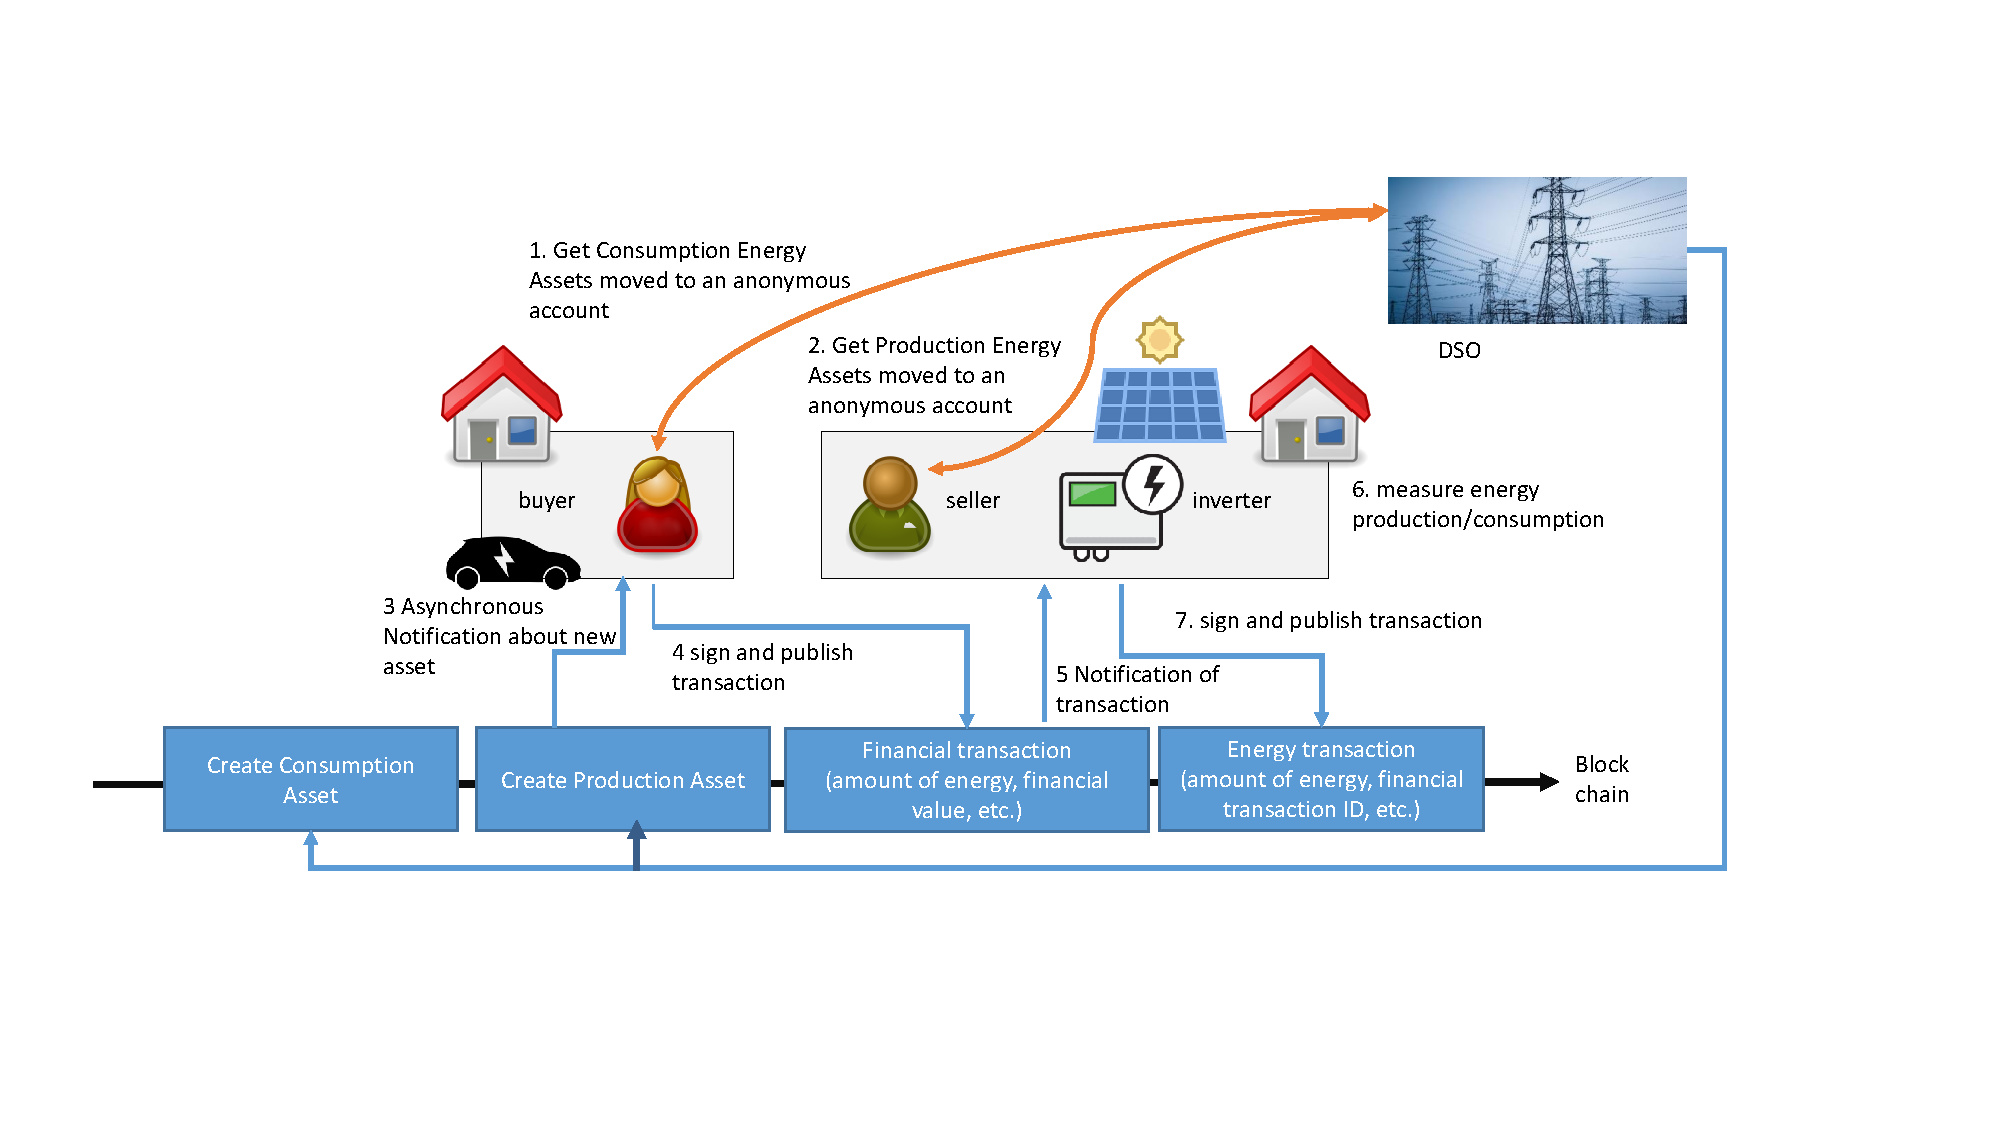
\includegraphics[width=\textwidth]{petra.pdf}
\caption{The sequence of activities in PETra. The orange arrows show off-block chain communication and blue arrows show transactions on block-chain. Producers and consumers request the DSO to allocate the energy production and consumption assets to blockchain. The consumers receive asynchronous notification about offers from producers. Thereafter, they can finalize transaction. The energy transfer happens at a later time and is also recorded in the chain. Financial transactions are also done on the blockchain. These financial transactions are later tallied with the energy transactions.}\label{fig:petrasequence}
\end{figure*}

There is a systematic pattern emerging in the domain of Internet of Things which requires transactional capabilities. Examples include transactive ride-share systems \cite{yuan2016towards}, transactive health-care systems \cite{azaria2016medrec}, and transactive energy systems described earlier in this section. As shown in Figure \ref{fig:components}, there are three separate layers of this transaction. The first layer is the distributed ledger, which is responsible for keeping track of all log of all events of interest; in the energy domain these events are trades, energy transfer and financial transactions. In case of health care domain, the events record the time of access of the health care data. The data itself is not stored in the block-chain due to the size and privacy issues. Rather, the data is stored in the second layer, which can be implemented by either a cloud or a decentralized storage service like Storj\footnote{https://storj.io/}. The third layer is the IoT layer, which is responsible for sensing and control. This third layer is typically implemented using messaging middlewares like MQTT, DDS, etc. 

\definecolor{CustomBlue}{RGB}{88, 154, 214}
\definecolor{CustomOrange}{RGB}{238, 124, 33}

\begin{figure}
\centering
\resizebox {\columnwidth} {!} {
\centering
\begin{tikzpicture}[x=1.5cm, y=1.8cm, font=\small,
  Component/.style={fill=white, draw, align=center, rounded corners=0.1cm, drop shadow={shadow xshift=0.05cm, shadow yshift=-0.05cm, fill=black}},
  Connection/.style={<->, >=stealth, shorten <=0.15cm, shorten >=0.15cm, very thick, CustomOrange}]

\foreach \pos/\name in {0/pros1, 0.8/pros2, 1.6/pros3} {
  \node [Component] (\name) at (\pos - 4, \pos) {\texttt{IoT Device, geth}};
}

%\node [Component] (dso) at (-1, 2.6) {\texttt{IoT device, geth}};

\fill [fill=black!10] (90:1.5) -- (200:1.5) -- (340:1.5) -- (90:1.5);

\foreach \pos in {90, 200, 340} {
  \node [Component] at (\pos:1.5) {Ethereum\\miner (\texttt{geth})};
}

\node [Component, dotted] (contract) at (0, 0) {Smart contract\\(\texttt{Blockchain})};

\draw [Connection, bend left=0] (pros1) to (pros2);
\draw [Connection, bend left=0] (pros2) to (pros3);
\draw [Connection, bend left=-60] (pros3) to (pros1);

%\draw [Connection, CustomBlue, bend right=15] (dso) to (contract);
\draw [Connection, CustomBlue, bend right=0] (pros1) to (contract);
\draw [Connection, CustomBlue, bend right=0, , shorten <=0.5cm] (pros2) to (contract);
\draw [Connection, CustomBlue, bend right=0] (pros3) to (contract);

\node [Component, minimum width=10.25cm, minimum height=0.7cm] at (-1.39, -1.6) {Decentralized storage service};
\draw [Connection] (-3.2, -1.35) -- (-3.2, -0.32)  node [midway, right,black] {bulk data};
\draw [Connection, CustomBlue, ->] (0, -1.35) -- (0, -0.27)  node [midway, right, align=left, black, yshift={-0.1cm}] {meta\\[-0.2em]data};
\end{tikzpicture}
}
\vspace{-0.1in}
\caption{Components of IoT Blockchain pattern. Typically the IoT devices communicate with each other over a messaging middleware (red arrows). They also communicate with blockchain and smart contracts  (blue arrows) through clients, for example the Ethereum geth client. The miners are entities responsible for validating the events/transactions. %The distributed storage service is not shown in the figure.
}
\vspace{-0.1in}
\label{fig:components}
\end{figure}




The key aspect of this pattern is the tight integration of distributed  messaging patterns between actors and the blockchain-based communication network used for transferring transactional information. For example, in the transactive energy domain,  PETra, described in \cite{Laszka17}, involves the interactions between distribution system operator, prosumer, and a smart contract. The smart contract is  responsible for keeping track of the energy and financial assets enabling prosumers to post trade offers and exchange assets when another prosumer decides to accept.


The  algorithm of PETra uses quantised energy asset tokens\footnote{There are two kinds of energy tokens: Energy Production Asset and Energy Consumption Asset. Token attributes include power and time interval for which the token is valid.} that can represent the non-negative amount of power to be produced or consumed (for example, measured in watts),  the time interval in which energy is to be produced (or consumed) and the  last time interval in which energy is to be produced (or consumed) (Figure \ref{fig:petrasequence} describes the full sequence of activity). These assets are withdrawn and submitted to anonymized accounts on behalf of prosumers by the distribution system operator, which is also responsible for validating that the specific prosumer has the  energy capacity for feasible trades given the assets. Once the DSO posts the assets into the blockchain, prosumers can trade between themselves using these quantised assets and anonymized addresses, hiding their identity from each other. The DSO is also responsible for releasing and managing the transfer of currencies, which are represented by financial assets, which is  simply an unsigned integer value, denominated in a fiat currency. In this workflow, there are both on- and off-blockchain communications between DSO and prosumer. The off-blockchain communication is required to request the transfer of assets. On-blockchain communication occurs via filters that track the posting of assets. Similarly, prosumers also communicate which each other via blockchain to indicate when an offer has been posted and when a transaction has cleared. 

While all of the transactive IoT systems require communication and transactional anonymity there are domain-specific requirements and challenges that must be considered.  These characteristics and requirements guide us in the description of the anonymization architecture that we describe in the rest of this paper. Specifically, these characteristics are as follows: 
 (1) transactions in a microgrid must clear in bounded time and any errors must be detected\footnote{Energy trades that have an impact on real-time control (e.g., selling energy production for the near future) must be permanently recorded on the ledger \emph{in time} since grid control signals cannot be delayed.}, (2) typically, there is a dedicated communication channel available in a microgrid that connects the prosumers and the distribution system operator, (3) the set of participants in the network are fixed and known ahead of time. Thus, a discovery procedure is typically not required, and (4) even though all the transactions are anonymous there is still a need for maintaining associativity of properties like maximum generation capacity\footnote{To prevent destabilization of the grid, a producer should not be allowed to bid more than its maximum generation capacity.}, reputation scores to prosumers as they participate in trades to maximize the likelihood of success, while reducing the likelihood of jeopardizing the stability of the microgrid\footnote{A prosumer with low reputation score might have a history of not fulfilling the energy transfer obligations}. In the next two sections, we describe the mechanisms for implementing communication and transaction anonymity in this workflow.



% This section describes a basic system model of transactive IoT
% microgrids and formulates security, safety, and privacy requirements.
% A microgrid is a collection of prosumers (residential nodes) that are
% arranged within the same distribution feeder and support exchange of
% power between them. A prosumer node includes a smart
% inverter and a smart meter, which control the flow of power into and
% out of the prosumer. A microgrid also contains a set of nodes that are responsible for isolating faults on the feeder.  The
% \emph{Distribution System Operator} (DSO) operates %a set of
% switching nodes to control the connection of the microgrid to the rest
% of the distribution system. The DSO is responsible for regulating the
% net electric power into and out of the microgrid. Starting from this
% model, we next introduce the transactive microgrid model.

% \subsection{Transactive Microgrid System Model}
% \Abhishek{This is the perfect paragraph to define transactive
%   microgrid as a special application of IoT spread over a large
%   area. Perhaps we can find a citation that makes this point.}  We
% describe a basic system model of decentralized transactive IoT
% microgrids.  We discuss the following components: a distributed ledger
% for recording transactions, a bid storage service that facilitates
% finding trade partners, a microgrid controller for regulating the
% microgrid load, and smart meters for measuring the prosumers' energy
% production and consumption.


% \begin{figure}[h!]
% \center
% \begin{tikzpicture}[x=8cm, y=0.7cm, font=\small,
%   nodeStyle/.style={rounded corners=0.1cm, drop shadow={shadow xshift=0.05cm, shadow yshift=-0.05cm, fill=black}}
% ]
% \draw [nodeStyle, fill=red!10]  (0, 1.65) rectangle    (1, 2.25) node [midway, align=center] {Communication anonymity (e.g., onion routing)};

% \draw [nodeStyle, fill=blue!10] (0, 2.4) rectangle    (1, 3.0) node [midway, align=center] {Distributed ledger (e.g., blockchain)};

% \draw [nodeStyle, fill=red!10]  (0, 3.15) rectangle (0.45, 4.05) node [midway, align=center] {Transaction anonymity\\[-0.2em](mixing service)};
% \draw [nodeStyle, left color=blue!10, right color=red!10] (0.47, 3.15) rectangle (0.72, 4.05) node [midway, align=center] {Bid storage};
% \draw [nodeStyle, left color=blue!10, right color=red!10] (0.74, 3.15) rectangle (1, 4.05) node [midway, align=center] {Active\\[-0.2em]smart meter};

% \draw [nodeStyle, fill=red!10] (0, 4.2) rectangle (0.49, 5.1) node [midway, align=center] {Anonymous trading\\[-0.2em]workflow for prosumers};
% \draw [nodeStyle, fill=blue!10] (0.51, 4.2) rectangle (1, 5.1) node [midway, align=center] {Microgrid controller};
% \end{tikzpicture}
% \caption{Architecture of a decentralized transactive microgrid with \mbox{PETra}.}
% \label{fig:softwareArchitecture}
% \end{figure}

% Figure~\ref{fig:softwareArchitecture} shows a decentralized
% transactive microgrid with PETra.  
% In this figure, components marked in blue are basic elements of the decentralized transactive microgrid,
% while components marked in red are added (or extended) by PETra.

% \subsubsection{Distributed Ledger}
% Distributed ledger technologies, usually summarized under the term "blockchain" provide a distributed, decentrilized and highly fault tolerant database to facilitate secure transactions (messages) between all participants, and immutably store these transactions.  

% \subsubsection{Bid Storage Service}
% In large networks of prosumers it might make sense -for the sake of scalability- to offer platform services where bids and calls for trades can be published.

% \subsubsection{Microgrid Controller (Distribution System Operator)}
% The DSO includes a controller that regulates the total load on the microgrid and from the microgrid to the distribution system. The controller first predicts load in the
% microgrid based on (1) bids and asks in the bid storage and (2)
% outstanding energy trades in the ledger.  By combining this
% information with the prediction for the rest of the grid, the
% controller produces a control signal that specifies how much the
% microgrid load should be decreased or increased. Based on this
% signal, the controller then updates the price policy for the microgrid
% to influence energy production and consumption.  We also assume the
% presence of a secondary controller that balances voltage and frequency
% in the microgrid.

% \subsubsection{Smart Meters}
% To measure the prosumers' energy production and consumption, a smart
% meter must be deployed at each prosumer.  As with any blockchain-connected device, it needs to be tamper-resistant, in this case to prevent electricity theft. 

% \subsection{Requirements}
% We now discuss the security, safety, and privacy requirements that
% must be satisfied by a transactive energy IoT system.

% \subsubsection{Security}
% Security requirements ensure primarily that prosumers are billed
% correctly, but they also provide necessary prerequisite properties for
% safety.
% More specifically, they require that
% \begin{itemize}[noitemsep,topsep=-\parskip]
% \item prosumers are billed correctly based on the energy prices set by
%   the DSO, their energy trades, and their actual energy production and
%   consumption measured by the smart meters,
% \item prosumers or outside attackers cannot change microgrid
%   regulatory policies that are set by the DSO, 
% \item prosumers cannot back out of trades unilaterally, and they
%   cannot tamper with other prosumers' trading or bidding,
% \item financial and physical impact of compromised or faulty nodes is
%   limited, and nodes can be banned by the DSO. 
% \end{itemize}

% \subsubsection{Safety}
% A large gap between the aggregate production and consumption threatens the stability of not only the microgrid but also the main
% power grid.  Therefore, prosumers should not be able to trade large
% amounts of energy that they are unlikely to deliver.
% Specifically, we require that 
% \begin{itemize}[noitemsep,topsep=-\parskip]
% \item the net amount of energy sold (or bought) by a prosumer is upper
%   bounded (by a limit set by the DSO), where the net amount of
%   energy sold is the difference between the amount of energy sold and
%   bought by the prosumer, and the net amount of energy bought is
%   defined analogously. %,
% \Aron{If we have space, add back the safety requirement on the bid storage (and also add back the relevant parts of the description of the trading workflow and the ``analysis.''}
% %\item the energy bids and asks posted by a prosumer are limited in a similar way.
% \end{itemize}
% In practice, the DSO can set the limits based on the prosumers' production and consumption capacities.

% \subsubsection{Privacy} 
% Privacy requirements ensure that the prosumers' privacy is not
% compromised when they participate in energy trading.  We use
% non-transactive smart metering as a baseline, and we require that
% the transactive system does not leak any additional information
% compared to this baseline.  More specifically, we require that
% \begin{itemize}[noitemsep,topsep=-\parskip]
% \item the corresponding smart meter and DSO shall gain and retain as little information regarding the energy produced, consumed, bought and sold by a prosumer,
% \item only the prosumer may know which bids and asks it has posted,
%   and no one can know who traded energy with whom.
% \end{itemize}




\section{Proposed System}

In this section, we describe our solution for providing privacy for prosumers without compromising the safety and security of the microgrid.
Figure~\ref{fig:softwareArchitecture} shows a high-level overview of the architecture of our solution.

\begin{figure}[h!]
\center
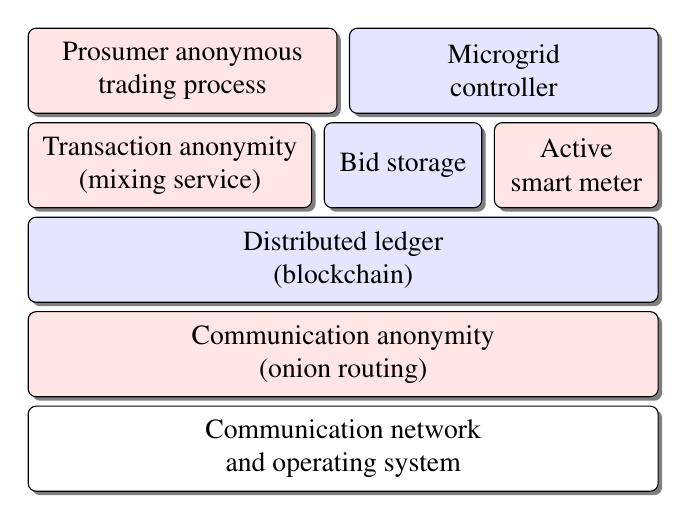
\begin{tikzpicture}[x=8cm, y=1.2cm,
  nodeStyle/.style={rounded corners=0.1cm, drop shadow={shadow xshift=0.05cm, shadow yshift=-0.05cm, fill=black}}
]
\draw [nodeStyle, fill=white]   (0, 0) rectangle    (1, 0.9) node [midway, align=center] {Communication network\\and operating system};

\draw [nodeStyle, fill=red!10]  (0, 1) rectangle    (1, 1.9) node [midway, align=center] {Communication anonymity\\(onion routing)};

\draw [nodeStyle, fill=blue!10] (0, 2) rectangle    (1, 2.9) node [midway, align=center] {Distributed ledger\\(blockchain)};

\draw [nodeStyle, fill=red!10]  (0,    3) rectangle (0.45, 3.9) node [midway, align=center] {Transaction anonymity\\(mixing service)};
\draw [nodeStyle, fill=blue!10] (0.47, 3) rectangle (0.72, 3.9) node [midway, align=center] {Bid storage};
\draw [nodeStyle, fill=red!10 ] (0.74, 3) rectangle (1,    3.9) node [midway, align=center] {Active\\smart meter};

\draw [nodeStyle, fill=red!10] (0,    4) rectangle (0.49, 4.9) node [midway, align=center] {Prosumer anonymous\\trading process};
\draw [nodeStyle, fill=blue!10] (0.51, 4) rectangle (1,    4.9) node [midway, align=center] {Microgrid\\controller};
\end{tikzpicture}
\caption{High-level architecture of the proposed solution. Components marked red are introduced to provide privacy in a safe and secure manner. Components marked in blue are typical elements of a decentralized transactive microgrid.}
\label{fig:softwareArchitecture}
\end{figure}

\begin{figure*}[h]
\center
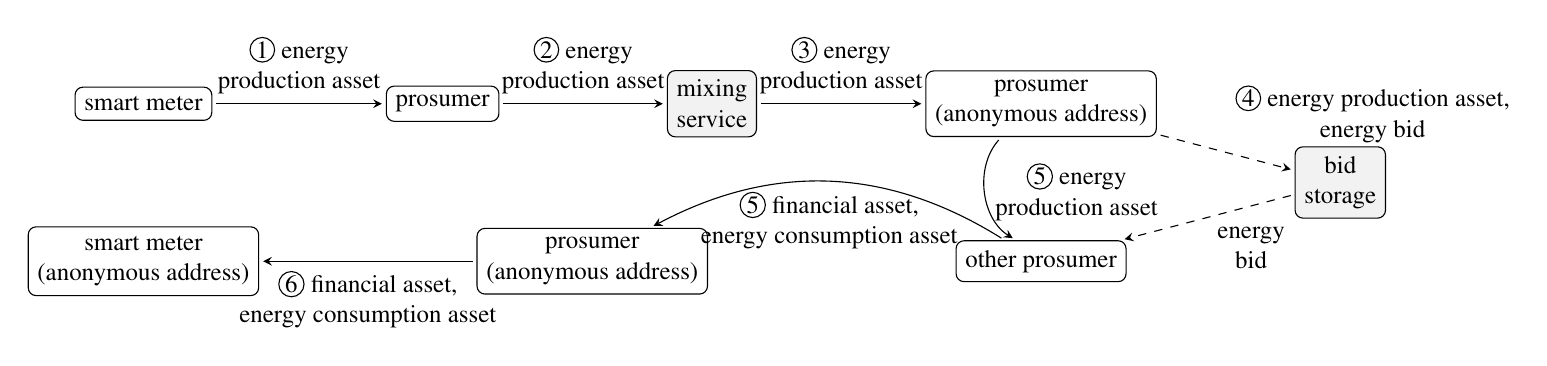
\begin{tikzpicture}[x=3.8cm, y=2cm, font=\small,
  system/.style={draw, align=center, rounded corners=0.1cm, fill=black!5},
  entity/.style={draw, align=center, rounded corners=0.1cm},
  asset/.style={midway, align=center},
  transfer/.style={->, >=stealth, shorten <=0.05cm, shorten >=0.05cm},
]
%\node[entity] (smartmeter) at (0.75, 0.5) {smart\\meter};
%\node[entity] (prosumer1) at (1.25, 1) {prosumer};
%\node[system] (mixing1) at (2, 1) {mixing\\service};
%\node[entity] (prosumer2) at (3, 1) {prosumer\\(alternative address)};
%\node[system] (bidstorage) at (4, 1) {bid\\storage};
%\node[entity] (partner) at (4, 0) {other prosumer};
%\node[entity] (prosumer3) at (3, 0) {prosumer\\(alternative address)};
%\node[system] (mixing2) at (2, 0) {mixing\\service};
%\node[entity] (prosumer4) at (1.25, 0) {prosumer};
\node[entity] (smartmeter) at (0, 1) {smart meter};
\node[entity] (prosumer1) at (1, 1) {prosumer};
\node[system] (mixing1) at (1.9, 1) {mixing\\service};
\node[entity] (prosumer2) at (3, 1) {prosumer\\(anonymous address)};
\node[system] (bidstorage) at (4, 0.5) {bid\\storage};
\node[entity] (partner) at (3, 0) {other prosumer};
\node[entity] (prosumer3) at (1.5, 0) {prosumer\\(anonymous address)};
\node[entity] (smartmeter2) at (0, 0) {smart meter\\(anonymous address)};

%\draw[transfer] (smartmeter) -- node [asset, above left] {energy\\production asset} (prosumer1);
%\draw[transfer] (prosumer1) -- node [asset, above] {energy\\production asset} (mixing1);
%\draw[transfer] (mixing1) -- node [asset, above] {energy\\production asset} (prosumer2);
%\draw[transfer, dashed] (prosumer2) -- node [asset, above] {energy production asset,\\energy bid} (bidstorage);
%\draw[transfer, dashed] (bidstorage) -- node [asset, right] {energy\\bid} (partner);
%\draw[transfer, bend right=15] (partner) to node [asset, below] {financial asset,\\energy\\consumption asset} (prosumer3);
%\draw[transfer, bend right=7.5] (prosumer2) to node [asset, above right] {energy\\prod. asset} (partner);
%\draw[transfer] (prosumer3) -- node [asset, below] {financial asset,\\
%energy consumption asset} (mixing2);
%\draw[transfer] (mixing2) -- node [asset, below] {financial asset,\\energy consumption asset} (prosumer4);
%\draw[transfer] (prosumer4) -- node [asset, below left] {financial\\asset} (smartmeter);

\draw[transfer] (smartmeter) -- node [asset, above] {\circled{1} energy\\production asset} (prosumer1);
\draw[transfer] (prosumer1) -- node [asset, above] {\circled{2} energy\\production asset} (mixing1);
\draw[transfer] (mixing1) -- node [asset, above] {\circled{3} energy\\production asset} (prosumer2);
\draw[transfer, dashed] (prosumer2) -- node [asset, above right] {\circled{4} energy production asset,\\energy bid} (bidstorage);
\draw[transfer, dashed] (bidstorage) -- node [asset, below right] {energy\\bid} (partner);
\draw[transfer, bend right=30] (partner) to node [asset, below] {\circled{5} financial asset,\\energy consumption asset} (prosumer3);
\draw[transfer, bend right=50] (prosumer2) to node [asset, right] {\circled{5} energy\\production asset} (partner);
\draw[transfer] (prosumer3) -- node [asset, below] {\circled{6} financial asset,\\
energy consumption asset} (smartmeter2);
\end{tikzpicture}
\caption{Simplified overview of the flow of assets from the perspective of a prosumer who sells energy. Note that in order to prevent de-anonymization, a prosumer should use multiple addresses and multiple rounds of mixing.}
\label{fig:sellFlow}
\end{figure*}

\subsection{Overview of the Trading Process}
We begin with a semi-formal description of the energy trading process from the prosumers' perspective.
In subsequent subsections, we will describe the assets, transactions, and services in our system in more detail.

First, consider a prosumer who would like to sell energy to another prosumer (this case is illustrated in Figure~\ref{fig:sellFlow}).
As its very first step, the prosumer obtains an \emph{energy production asset} from its smart meter.
An energy production asset represents a permission to sell a certain amount of energy, and it is used to enforce safety requirements.
If the prosumer has sufficient unsold production capacity, the smart meter creates and transfers a production asset to the prosumer using a \emph{smart meter transaction} \circled{1}, which is recorded on the distributed ledger.

At this point, the production asset can still be traced back to the prosumer since the ledger is public.
To achieve anonymity, the prosumer transfers the production asset to a \emph{mixing service} using an \emph{energy and financial transaction} \circled{2}, which is also recorded on the distributed ledger.
In turn, the mixing service transfers the production asset to an \emph{anonymous address} \circled{3}\todo{We should probably insert a good definition here for reader who are unfamiliar with blockchain transactions.}, which is randomly generated and controlled by the prosumer.
Since the mixing service transfers assets from multiple prosumers to multiple anonymous addresses at the same time, and the anonymous addresses were chosen at random by the prosumers, the assets cannot be traced back to the original prosumers after mixing.\footnote{Note that prosumers should divide their assets between multiple anonymous addresses; otherwise, each asset might be traced back to its prosumer based on the amount of energy that it contains.}

Now, the prosumer can engage in energy trading anonymously.
To find a trade partner, it can either post an \emph{energy bid} on the bid storage, or simply search the storage for an acceptable \emph{energy ask}.
To post an energy bid, the prosumer first proves to the storage service -- without revealing its original identity -- that it owns a production asset stored at an anonymous address.
It can then post the energy bid \circled{4}, which contains an anonymous communication address\footnote{We discuss communication anonymity later.}, a price, and a reference to the production asset.
If another prosumer, who would like to buy energy, finds the bid acceptable, it can contact the selling prosumer at the communication address given by the bid.

The seller and buyer can execute the trade by creating an energy and financial transaction together \circled{5}, and recording it on the ledger.
This transaction transfers the production asset from the seller to the buyer, and a \emph{financial asset} and an \emph{energy consumption asset} from the buyer to the seller.
A financial asset represents a certain amount of money, while a consumption asset represents a permission to buy a certain amount of energy, which is used to enforce safety requirements similarly to production assets.

Finally, the selling prosumer deposits the financial and consumption assets to its smart meter using an energy and financial transaction.
To ensure that the prosumer remains anonymous, it transfers the assets to an anonymous address that is randomly generated and controlled by the smart meter \circled{6}.
Once the smart meter has received the assets, it credits the financial amount to and deducts the energy amount from the prosumer, for billing purposes.
Note that in order to enforce safety requirements, the prosumer must always deposit the same amount of consumption assets as the amount of production assets obtained at the beginning; otherwise, unaccounted consumption assets might be used to trade excessive amounts.

Second, consider a prosumer who would like to buy energy from another prosumer.
Since the trading process is very similar to the case of the selling prosumer, we will discuss only the differences.
In the first step, the prosumer tries to obtain a financial asset and an energy consumption asset from its smart meter.
If the prosumer has the consumption capacity and good financial standing, the smart meter transfers the assets to the prosumer and adds the financial amount to the prosumer's bill.
After transferring the assets through a mixing service, the prosumer is ready to post an energy ask on the bid service.
To do so, it first proves the ownership of both the financial asset and the consumption asset to the service, and then posts the energy ask, which includes an anonymous communication address.
If a partner is found, the trade is executed as described before, the prosumer playing the role of the buyer.
Finally, the prosumer deposits the purchased energy production asset to the anonymous address of its smart meter,
which credits the energy amount to the prosumer, for billing purposes.
Note that if the prosumer has not used up the financial asset completely, then the remainder may also be deposited back to the smart meter.

\subsection{Timing}
The ability to specify points or intervals in time is crucial.
For example, control signals specify how the load should change at certain points in time, energy trades specify when energy will be consumed or produced, etc.
To facilitate processing signals and transactions, we divide time into fixed-length intervals, and specify points or periods in time using these discrete timesteps.
The length of the time interval is determined by mapping the timing assumptions of the power system to our platform.
%In our implementation, 
For example, the default length of the time interval may be 4 seconds, which corresponds to how frequently the control signal of the DSO typically changes.

\subsection{Transactions}

In the previous subsection, we gave an overview of how transactions are used in the trading process to transfer various assets.
Here, we detail the format of these transactions, and the rules that they have to satisfy to be valid and recorded on the ledger.
We also introduce and detail the format of regulatory transactions, which the DSO uses to regulate the microgrid.

\subsubsection{Timing}

The ability to specify points or intervals in time is crucial.
For example, control signals specify how the microgrid load should change at certain points in time, energy trades specify when energy will be consumed or produced, etc.
To facilitate processing signals and transactions, we divide time into fixed-length intervals, and specify points or periods in time using these discrete timesteps.
The length of the time interval is determined based on the timing assumptions of the physical power system.
For example, the default length of the time interval may be 4 seconds, which corresponds to how frequently the control signal of the DSO typically changes.
\Abhishek{We need to add citation here. I will add that tomorrow.}
\Abhishek{What about the deadline within which the transactions should finish? Do we need to say anything here?}
\Aron{Ideally, we should discuss the timing constraints of the ledger (probably when we introduce it), but we would first need to make space for this discussion.}

\subsubsection{Assets}

Before we can discuss transactions, we must define the format of three assets that these transactions may transfer.
First, an \emph{energy production asset} (EPA) is defined by
\begin{compactitem}
\item \field{power}: non-negative amount of power to produced (for example, measured in watts),
\item \field{start}: first time interval in which energy is to be produced,
\item \field{end}: last time interval in which energy is to be produced.
\end{compactitem}
Second, an \emph{energy consumption asset} (ECA) is defined by the same fields; however, for this asset, the fields define energy consumption instead of production.
Finally, a \emph{financial asset} (FA) is defined by a single non-negative number \field{amount}, which can be denominated in either a fiat currency (e.g., US dollars) or a cryptocurrency.

\subsubsection{Energy and Financial Transactions}

Energy and financial transactions transfer energy and financial assets from one address to another.
Prosumers use these transactions for multiple purposes: to trade energy by exchanging assets with other prosumers, to prove to the bid storage that they have production or consumption capacity, to hide their identity by transferring assets to and from mixing services, and to deposit assets at their smart meter.
%
An energy and financial transaction contains the following fields:
\begin{compactitem}
\item \field{EPA\_in}: list of EPA inputs, each of which is defined by
\begin{itemize}[leftmargin=0.5em,nosep]
\item \field{out}: reference to an EPA output of a previous transaction,
\item \field{sig}: signature for referenced output,
\end{itemize}
\item \field{ECA\_in}: list of ECA inputs, each of which is defined by
\begin{itemize}[leftmargin=0.5em,nosep]
\item \field{out}: reference to an ECA output of a previous transaction,
\item \field{sig}: signature for referenced output,
\end{itemize}
\item \field{FA\_in}: list of FA inputs, each of which is defined by
\begin{itemize}[leftmargin=0.5em,nosep]
\item \field{out}: reference to an FA output of a previous transaction,
\item \field{sig}: signature for referenced output,
\end{itemize}
\item \field{EPA\_out}: list of EPA outputs, each of which is defined by
\begin{itemize}[leftmargin=0.5em,nosep]
\item \field{EPA}: an energy production asset,
\item \field{address}: address to which EPA is transferred,
\end{itemize}
\item \field{ECA\_out}: list of ECA outputs, each of which is defined by
\begin{itemize}[leftmargin=0.5em,nosep]
\item \field{EPA}: an energy consumption asset,
\item \field{address}: address to which ECA is transferred,
\end{itemize}
\item \field{FA\_out}: list of FA outputs, each of which is defined by
\begin{itemize}[leftmargin=0.5em,nosep]
\item \field{EPA}: a financial asset,
\item \field{address}: address to which FA is transferred,
\end{itemize}
\end{compactitem}
This transaction transfers the assets specified in the input lists to the addresses specified in the output lists. 
Note that assets may be divided or combined, as the input and output lists may differ in length.

An energy and financial transaction is valid (and can be recorded on the ledger) if the following three conditions hold.
\begin{itemize}[noitemsep,topsep=-\parskip]
\item None of the outputs referenced by the inputs have been spent by a transaction that has been recorded on the ledger.
\item All of the signatures are valid, which ensures that only the current owner can transfer an asset.
\item For each asset type (and for each timestep), the sum of inputs and outputs is equal.
For example, in the case of energy production assets, the condition is
\begin{align*}
& \forall t: \sum_{\substack{out \,\in\, \field{EPA\_out}:\\out.\field{EPA}.\field{start} \leq t \leq out.\field{EPA}.\field{end}}} out.\field{EPA}.\field{power} \nonumber \\
& = \sum_{\substack{in \,\in\, \field{EPA\_in}:\\in.\field{out}.\field{EPA}.\field{start} \leq t \leq in.\field{out}.\field{EPA}.\field{end}}} in.\field{out}.\field{EPA}.\field{power}  .
%
%& \forall t: \sum_{out \in \field{EPA\_out}} out.\field{EPA}.\field{power} \cdot 1_{\left\{out.\field{EPA}.\field{start} \leq t \leq out.\field{EPA}.\field{end}\right\}} \nonumber \\
%& = \sum_{in \in \field{EPA\_in}} in.\field{out}.\field{EPA}.\field{power} \cdot 1_{\left\{in.\field{out}.\field{EPA}.\field{start} \leq t \leq in.\field{out}.\field{EPA}.\field{end}\right\}} ,
\end{align*}
%where $1_x$ is equal to $1$ if $x$ is true, and it is $0$ otherwise.
%\begin{equation}
%\forall t: \sum_{out \in \left\{out' \middle| out' \in \text{ EPA outputs} \wedge out'.EPA.start \leq t \leq out'.EPA.end\right\}} out.EPA.Power = \sum_{in \in \left\{in' \middle| in' \in \text{ EPA inputs} \wedge in'.EPA.start \leq t \leq in'.EPA.end\right\}} in.EPA.Power .
%\end{equation}
The conditions for consumption and financial assets can be described formally in similar ways.
\end{itemize}
%If a transaction submitted to the ledger is valid, it will be permanently recorded.

\subsubsection{Smart-Meter Transactions}

Prosumers use smart-meter transactions to withdraw energy and financial assets from their own smart meters, before they engage in trading.
%
A transaction contains the following fields:
\begin{compactitem}
\item \field{EPA\_out}: list of EPA outputs (see above),
\item \field{ECA\_out}: list of ECA outputs (see above),
\item \field{FA\_out}: list of FA outputs (see above),
\item \field{id}: smart meter's identifier,
\item \field{sig}: smart meter's signature over the transaction.
\end{compactitem}
This transaction creates and transfers the assets to the prosumer's addresses, which are specified in the output lists.

The smart meter signs the transaction only if the prosumer is allowed to withdraw these assets.
More specifically, the amount of withdrawn assets can never exceed certain limits that are set by the DSO.
For example, in the case of EPA, the following condition must be satisfied for prosumer $i$:
\begin{equation}
\forall t: \sum_{tr \,\in\, \field{TR}_i} \sum_{\substack{out \,\in\, tr.\field{EPA\_out}:\\out.\field{EPA}.\field{start} \leq t \leq out.\field{EPA}.\field{end}}} out.\field{EPA}.\field{power} < \field{MAXEPA}_i ,
\end{equation}
where $\field{TR}_i$ is the set of smart-meter transactions recorded for prosumer $i$ and $\field{MAXEPA}_i$ is the withdrawal limit.
The condition for consumption assets is similar, based on a limit $\field{MAXECA}_i$.
For financial assets, the smart meter takes into account the amounts withdrawn and deposited, as well as the outside bill payments to the DSO.

\Aron{To address malfunctioning or compromised smart meters, we could also impose a limit on withdrawals.}
A transaction is valid if the following two conditions hold.
\begin{itemize}[noitemsep,topsep=-\parskip]
\item The smart meter identified in the transaction has been authorized by a regulatory transaction that was previously recorded on the ledger.
\item The smart meter's signature is valid (for public key, see regulatory transactions).
\end{itemize}

\subsubsection{Regulatory Transactions}

The DSO uses regulatory transactions for two purposes: to manage the set of authorized smart meters and to change the price policy.
%First, to change the set of smart meters that are authorized to sign transactions, the DSO authorizes or bans individual smart meters.
First, whenever a new smart meter is installed, the DSO notifies the microgrid by authorizing the device using a regulatory transaction.
Similarly, whenever a smart meter is deactivated (e.g., because service is stopped or the device is believed to be malfunctioning or compromised), the DSO notifies the microgrid by banning the device.
Second, to influence microgrid load, the DSO can set a price policy, which includes a price at which prosumer may buy energy from the DSO and a price at which they may sell energy to the DSO.

A regulatory transactions contain the following fields:
\begin{compactitem}
\item \field{authorize}: list of smart meters to be authorized, each of which is defined by
\begin{compactitem}
\item \field{id}: identifier of the smart meter,
\item \field{pubkey}: public key of the smart meter,
\end{compactitem}
\item \field{ban}: list of identifiers of smart meters to be banned, 
\item \field{priceConsumption}: price at which DSO sells energy,
\item \field{priceProduction}: price at which DSO buys energy,
\item \field{time}: timestep after which authorizations, bans, and price changes should take effect,
\item \field{sig}: DSO's signature over the transaction.
\end{compactitem}

A regulatory transaction of this type is valid if %the following two conditions hold:
%\begin{compactitem}
%\item 
\field{timestep} is not in the past and % specified in the transaction is in the future.
%\item 
the DSO's signature is valid.
%\end{compactitem}
%
The active prices for timestep $t$ are given by the last regulatory transaction recorded on the ledger whose \field{time} is less than $t$.
Similarly, regulatory transactions that are recorded on the ledger later override the authorizations and bans of earlier transactions.



\subsection{Services}

In this subsection, we describe the various services that are implemented in our system. %on which transactions are built and which build on transactions.
We have already discussed the distributed ledger, which permanently stores valid transactions.
Now, we will introduce anonymous communication service, mixing service for transaction anonymity, anonymous bid storage, and smart-meter based billing.\Aron{Revise list based on final organization!}

\subsubsection{Communication Anonymity}
Firstly, we must provide an anonymous communication layer, on which we can build all the other services in our system.
Without this communication layer, transactions and bids could be easily de-anonymized based on their sources' network identifiers (e.g., IP or MAC addresses).

We can employ well-known and widely used techniques for anonymous communication, such as \emph{onion routing}~\cite{reed1998anonymous}.
To build an onion network, the smart meters, prosumers, and other devices can act as onion routers, and the list of onion routers in a microgrid can be published on the ledger.
In practice, this service can built on 
%In our first implementation, we can use
 the free and open-source Tor software with private Directory Authorities.
In this case, anonymous communication addresses in bids and asks correspond to public-keys that identify Tor hidden services.
% ritter.vg: "run your own tor network"
% https://ritter.vg/blog-run_your_own_tor_network.html

\subsubsection{Transaction Anonymity}
Communication anonymity is necessary for anonymous trading, but it is not sufficient: if prosumers used their own accounts to transfer assets, trades would not be anonymous.
Fortunately, most distributed ledgers allow users to easily generate new addresses\footnote{The usage of the term \emph{address} varies between distributed ledgers, but our system could be implemented using any popular ledger, such as Bitcoin and Ethereum. 
Specifically, we use the term address to denote a possible destination for asset transfers. 
Assets transferred to an address can be used only by someone who knows the private key of the address (typically, the one who generated the address).} 
at random.
Since these addresses are generated randomly, they are anonymous in the sense that no one can tell who generated them.
However, if prosumers simply transferred assets to these addresses, they could be easily de-anonymized by tracing the assets back to the prosumers.

To prevent this, prosumers transfer assets to their anonymous addresses through a \emph{mixing service}. 
The mixing service prevents tracing the assets back to their original owners by mixing together multiple incoming transfers and multiple outgoing transfers, thereby hiding the connections between the prosumers and the anonymous addresses.
In practice, a mixing service can be implemented using multiple approaches.
The simplest one is to use a \emph{trusted third party}, called a cryptocurrency tumbler, which can receive and send assets.
However, anonymity in this case depends on the trustworthiness and reliability of the third party, who could easily de-anonymize the addresses.
A more secure approach is to used decentralized protocols, such as CoinShuffle~\cite{ruffing2014coinshuffle} or Xim~\cite{bissias2014sybil}.
These protocols enable participants to mix assets with each other, thereby eliminating the need for a trusted third party, which would constitute a single point of failure.
Some newer cryptocurrencies, such as Zerocoin~\cite{miers2013zerocoin},  provide built-in mixing services, which are often based on cryptographic principles and proofs.

\begin{comment}
We must provide prosumers with the ability to create and publish transactions anonymously.
More specifically, prosumers should be able to purchase or sell energy without revealing their identity; however, these transaction must also be verifiable and enforceable.

We may achieve this goal using multiple approaches for blockchain transaction anonymity:
\begin{itemize}
\item Mixing services (also known as tumblers) mix potentially identifiable assets on a blockchain with others, thereby preventing tracing individual assets back to their original source. 
In our case, assets to be mixed include virtual balances of fiat currencies as well as energy production and consumption.
\item Cryptographic anonymity for transactions is provided, for example, by Zerocoin~\cite{miers2013zerocoin}. Similarly to mixing service, Zerocoin can prevent tracing assets on a blockchain.
\end{itemize}
Using the above techniques, we can enable prosumers to trade energy anonymously (i.e., without revealing their true identities), but at the same time prevent them from altering their energy or financial balances without a valid transaction.

However, we must also ensure that 1) smart meters know the amount of energy purchased or sold by their prosumer and 2) prosumers cannot purchase or sell more energy than their capacity.
To satisfy both of these constraints, all energy trades must start with the prosumer withdrawing a certain amount of energy production or consumption from its smart meter:
\begin{itemize}
\item If a prosumer wishes to sell energy, it must first withdraw an energy asset from its smart meter using a blockchain transaction.
This transaction must be signed by the smart meter, which enables the smart meter to 1) keep track of the amount of energy traded by the prosumer as well as to 2) enforce safety requirements by limiting the amount of energy that can be withdrawn.
\item If a prosumer wishes to buy energy, it must first withdraw an energy consumption asset from its smart meter in a way similar to withdrawing an energy production asset.
\end{itemize}
\end{comment}

\subsubsection{Bidding Anonymity}
Finally, we must provide prosumers with the ability to post energy bids and asks anonymously.
To this end, we create a storage for anonymous bids that is readable by all the prosumers in the microgrid.
Any prosumer may submit a bid to this storage; however, in order to do so, they must provide a zero-knowledge proof of owning the assets that are to be traded:
\begin{itemize}
\item To submit an energy sell bid, the prosumer must prove that it owns an energy production asset on the chain.
\item To submit an energy buy bid, the prosumer must prove that it own an energy consumption asset as well as financial assets on the chain.
\end{itemize}

\subsubsection{Billing}

The energy consumption balance $E_i^t$ of prosumer $i$ in timeslot~$t$ is
\begin{align*}
E_i^t = & \hphantom{+} \text{measured consumption} - \text{measured production} \\
 & + \text{EPA deposited by $i$} - \text{EPA withdrawn by $i$} .
\end{align*}
Notice that energy consumption assets are not necessary for billing, they are only used to enforce safety requirements.

The financial balance $F_i^t$ of prosumer $i$ in timeslot $t$, which is to be paid by the prosumer to the DSO, is
\begin{align*}
F_i^t = & \hphantom{+} \text{FA deposited by $i$ in $t$} - \text{FA withdrawn by $i$ in $t$} \\
 & + \begin{cases}
E_i^t \cdot \field{priceProduction} & \text{ if } E_i^t < 0 \\
- E_i^t \cdot \field{priceConsumption} & \text{ otherwise.} 
\end{cases}
\end{align*}

\TODO{discussion of microgrid control based on bids and trades? (update subsubsection title)}





%!TEX root = paper.tex
\section{Discussion}
\label{sec:discussion}

This section presents a semi-formal analysis of PETra and shows that
it satisfies the security, safety, and privacy requirements formulated
earlier.

\subsection{Security}
Satisfaction of the security requirements follows from:
\begin{itemize}[noitemsep,topsep=-\parskip]
\item immutability of transactions in the distributed ledger,
\item validity conditions of the transactions, which include
  conditions on both signatures and asset balances,
\item and tamper-resistance of smart meters.
\end{itemize}
Together, these properties ensure that only the right entities may
create and sign a transaction, that transactions adhere to the rules
of the trading workflow, and that transactions cannot be tampered
with.\footnote{Due to lack of space, we leave a detailed discussion
  and proof for future work.}

\subsection{Safety}
We now demonstrate that faulty or malicious prosumers cannot trade
excessive amounts of energy if normal prosumers follow the rules of
the trading workflow.  First, we can show that the net amount of
energy sold by prosumer $i$ for each timestep is at most
$\field{MAXEPA}_i$.  Due to the rules of the trading workflow, the gross amount of energy sold is less than or equal to the amount of EPA
obtained by prosumer $i$.
%
A prosumer can obtain EPA either by withdrawing from its smart meter
or by purchasing from another prosumer.  From its smart meter,
prosumer $i$ can withdraw at most $\field{MAXEPA}_i$.  Although the
prosumer may also buy EPA from another prosumer, this constitutes
buying energy, which decreases the net amount of energy sold with the
same amount.  Hence, the net amount of energy sold by prosumer $i$
cannot exceed $\field{MAXEPA}_i$.  By extending the argument, we can
show that the net amount of energy sold by a group of prosumers~$G$
cannot exceed $\sum_{i \in G} \field{MAXEPA}_i$.  Similarly, %we can
%show that
 the net amount of energy bought by a group of prosumers $G$
cannot exceed $\sum_{i \in G} \field{MAXECA}_i$.

%Using a similar argument, we can also show that the total amount of energy bids (or asks) posted at
%the same time by prosumer $i$ for each timestep is at most
%$\field{MAXEPA}_i + \field{MAXECA}_i$.  This limit is higher than for
%net energy sold or bought, since prosumer $i$ may purchase
%$\field{MAXECA}_i$ amount of EPA (or $\field{MAXEPA}_i$ amount of ECA)
%from other prosumers, and then post an energy ask (or bid) in the
%amount of $\field{MAXEPA}_i + \field{MAXECA}_i$.

\subsection{Privacy}
Due to our use of communication anonymity and mixing services, members
of a microgrid can observe only the amount of assets withdrawn by a
prosumer from its smart meter.  Since all trading transactions are
anonymous, they do not reveal the actual amount of assets traded by
the prosumer.  If a prosumer has not traded away all of its assets,
then it can also anonymously deposit the remainder to a random address
that was freshly generated by its smart meter. Even if a prosumer does
not wish to trade, it should always withdraw, mix, and deposit the
same amount of assets.  Otherwise, the lack (or varying amount) of
withdrawal would leak information.

As for the DSO, it receives the same information from the smart meter
as in a non-transactive smart grid (\emph{i.e.}, amount of energy
produced and consumed).  Since trading is anonymous, the DSO learns
only the financial balance of the prosumer, which is necessary for
billing.  However, we can provide an even higher-level of privacy.  In
particular, since price policies are recorded on the ledger (which the
smart meters may read), each prosumer's smart meter may calculate and
send the prosumer's monthly bill to the DSO, without revealing the
prosumer's energy consumption or production.  Meanwhile, the DSO can
still obtain detailed load information (including predictions) for the
microgrid from the bid storage and the trades recorded on the ledger.



%!TEX root = paper.tex
\section{Related Work}
\label{sec:related}

%In this section we describe the related research. It has been divided into two subsections to focus on blockchains, which we are using to implement the distributed ledger service described earlier, and other works on smart grid privacy concerns. 

%\subsection{Smart Grid and Meter Privacy}
% http://ieeexplore.ieee.org/abstract/document/5054916/
%McDaniel and McLaughlin discuss privacy challenges in smart grids~\cite{mcdaniel2009security}.
% https://arxiv.org/pdf/1108.2234.pdf
% https://pdfs.semanticscholar.org/cdf8/a5b6256823bca38a1d2347ab36f8e4a2ca94.pdf
% http://www.comm.toronto.edu/~akhisti/sm.pdf
% https://www.researchgate.net/profile/Georgios_Kalogridis/publication/224189766_Smart_Grid_Privacy_via_Anonymization_of_Smart_Metering_Data/links/541169510cf2b4da1bec4193.pdf
% https://arxiv.org/pdf/1305.0735.pdf
New privacy concerns arise with the continuing adoption of smart
grids. In addition to old and new security threats (such as energy
theft and smart-meter malware), McDaniel and McLaughlin discuss the
privacy concerns of energy usage profiling that smart grids could
potentially enable~\cite{mcdaniel2009security}. Several approaches
have been investigated as potential means to provide privacy
protections for smart grid users.

Some approaches look to the use of protocols and/or frameworks to help
protect privacy. Rajagopalan et al.\ use tools from information theory
to present a framework that abstracts both the privacy and the utility
requirements of smart-meter
data~\cite{rajagopalan2011smart,sankar2013smart}. Their framework
leads to a novel tractable privacy-utility tradeoff problem with
minimal assumptions. Efthymiou and Kalogridis describe a method for
securely anonymizing frequent electrical metering data sent by a smart
meter~\cite{efthymiou2010smart}. Their approach is based on the
observation that frequent metering data may be required by an energy
distribution network for operational reasons, but it may not
necessarily need to be attributable to a specific smart meter. The
authors describe a method that provides a third-party escrow mechanism
for authenticated anonymous meter readings, which are hard to
associate with a particular smart meter.

Other approaches, such as additional hardware components, are explored
for potential privacy gains. Varodayan and Khisti study using a
rechargeable battery for partially protecting the privacy of
information contained in a household's electrical load
profile~\cite{varodayan2011smart}. They show that stochastic battery
policies may leak 26\% less information than a best-effort policy,
which holds the output load constant whenever possible. Tan et
al.\ study privacy in a smart metering system from an information
theoretic perspective in the presence of energy harvesting and storage
units~\cite{tan2013increasing}. They show that energy harvesting
provides increased privacy by diversifying the energy source, while a
storage device can be used to increase both energy efficiency and
privacy.
% They show that there exists a trade-off between the information
% leakage rate and the wasted energy rate, and study the impact of the
% energy harvesting rate and the size of the storage device on this trade-off.

PETra extends this earlier work by (1) leveraging a decentralized IoT
system for transactive energy and (2) addressing the novel privacy
threat posed by trading. In particular, while earlier work protected
the prosumers' privacy from the DSO, PETra also protects it from other
prosumers, as well as outside attackers.

A key element of PETra is its ability to distribute information among
peers via blockchains.  As blockchain technology develops and matures,
new frameworks, services, and protocols are being developed to
leverage the distributed ledgers provided by blockchains. For example,
Hyperledger Fabric is a platform for distributed ledger solutions,
which was designed to support pluggable implementations of different
components~\cite{hyperledger2017fabric}.
%Bitcoin Lightning Network is
%decentralized system, in which transactions are sent over a network of
%micropayment channels, whose transfer of value occurs
%off-blockchain~\cite{poon2016bitcoin}. 
Since this paper focuses on the theoretical foundations of PETra, any
of these distributed ledgers provide the required capabilities.

%\Abhishek{Aron this section should end with a few sentence about how our approach fits in. Perhaps just a few sentences reworded from introduction will be sufficient}

\iffalse
\subsection{Blockchains as Distributed Ledgers}

As Blockchain technology continues to develop and mature, new
frameworks, services, and protocols are being developed to leverage
blockchain's distributed ledger. Microsoft offers Blockchain as a
Service (BaaS) on Azure. Additionally, Microsoft has Project Bletchley
as its architectural approach to building an Enterprise Consortium
Blockchain Ecosystem, introducing two new concepts: blockchain
middleware and a secure means for calling code or data outside a
SmartContract or blockchain called
cryptlets~\cite{gray2016introducing}. Hyperledger Fabric is a platform
for distributed ledger solutions, which was designed to support
pluggable implementations of different
components~\cite{hyperledger2017fabric}. Bitcoin Lightning Network is
decentralized system, in which transactions are sent over a network of
micropayment channels whose transfer of value occurs
off-blockchain~\cite{poon2016bitcoin}. Interledger is a protocol for
payments across payment systems, which enables anyone with accounts on
two ledgers to create a connection between
them~\cite{thomas_protocol}. Xu et al.\ discuss the use of two pools
of proxy agents, an agreement pool and a payment pool, to assist in
protection of privacy when using blockchain technologies for
transactions on tangible goods~\cite{Xu2017}.  \fi

%\url{https://geli.net/residential/}
%\url{https://www.greentechmedia.com/articles/read/geli-raises-7m-to-take-energy-storage-software-to-the-next-level}

%\url{http://ethembedded.com/}


\section{Conclusion}
\label{sec:concl}


% BALANCE COLUMNS
\balance{}

% REFERENCES FORMAT
% References must be the same font size as other body text.
\bibliographystyle{SIGCHI-Reference-Format}
\bibliography{references}

\end{document}

